\nnarticleheader{The Beauty of Newton’s First Law of Motion}{Mitav Nayak, Haverford '22}

\noindent
\begin{quotation}
\textit{Every body persists in its state of being at rest or of moving uniformly straight forward, except insofar as it is compelled to change its state by force impressed}
\begin{flushright}
Sir Isaac Newton
\end{flushright}
\end{quotation}

\noindent
\textbf{Introduction}

Above is Newton’s first law as written in 1687 in his book \emph{Principia Mathematica}, translated from his own Latin words; the law that seems to have redefined and refined human understanding of a previously hazy phenomenon: motion. However, while Newton is generally given credit for this discovery, it was really Galileo who first pieced together a clear understanding of motion with his law of inertia. Both laws essentially said the same thing: an object remains at motion or at rest unless acted upon by another force.

While all three of Newton’s laws are brilliant, I find the first to be perhaps the most intriguing. Nowadays, people seem to take the law for granted. We’ve heard it said—in some form or another—since elementary school. At this point, it almost seems \emph{obvious}. But it is not obvious. In fact, I would argue that it is almost counterintuitive: have \emph{you} ever seen an object stay in a state of motion for eternity?

\noindent
\textbf{The History of Motion}

This, the concept of an object staying in a state of motion for eternity, is what I find fascinating. For hundreds of years, physicists and philosophers had attempted to make sense of the concept of motion. Greek philosopher Aristotle was in many eyes one of the first to put forth ideas regarding motion; ideas that lingered for over a thousand years. Aristotle believed that there existed four elements—Earth, Water, Air, and Fire—and that motion was a result of objects attempting to reach their natural place. For example, he argued that smoke rises because it mostly consists of air, rain falls because it consists of water, and a rock falls to reach the Earth. This, I would argue, seems much more intuitive to most people. It’s no wonder the ideas were prevalent for such a long period of time.

When Galileo and Newton came along almost two thousand years later and redefined motion, physics was altered forever. One part of the law, the part that asserts an object will stay at rest unless acted upon, may not have come as too much of a shock to people. It was not necessarily “groundbreaking,” as Aristotle himself had argued something similar. He differentiated “natural motion” (i.e. water falling) with “violent motion,” explaining that motion against an object’s natural state—like picking up a rock from the ground—was the latter. He believed that a heavy rock would stay at rest forever in this “natural” state, unless someone exerted “violent motion” upon it. The other part of Newton’s law, however, was the novel and mind-blowing part, changing how people perceived an object’s “natural state.”

\noindent
\textbf{The Natural State of Motion}

People could not comprehend that an object may persist in a state of motion forever, largely because we do not see it occur on a day to day basis. In our lives, whenever we see an object start moving, it ultimately stops. Galileo and Newton’s discovery that an object could start moving and would naturally never stop seemingly went against real-life observations. But, if we look closely, there are examples of objects persisting—or “wanting” to persist—in a state of motion in real life. For example, when we slide a hockey puck on ice, it will continue skidding along for a long period of time. We know that it will eventually stop, as even the smoothest ice has at least some friction, meaning that there is in fact another force acting on the moving puck. But if we could imagine the puck in a completely frictionless ice rink, the law of inertia suggests the puck would continue in its state of motion for eternity. It would never slow down or stop. Another example of the law is an instance of sudden braking or acceleration in the vehicle. If we are traveling in a car and have to suddenly stop, or hit a brick wall, our body throws itself forward. While the car stops, our body “wants” to stay in its state of motion. If we suddenly accelerate from rest, our body flies backward against our seat, “wanting” to stay in a state of rest.

Before the law of inertia, people believed there was some force acting on an object in motion which caused it to continue moving. They would argue that the moving hockey puck has something acting on it that allows it to propel itself forward. It was hard to understand that, just like a still hockey puck will not move unless something impels it to, a moving hockey puck on frictionless ice will not stop unless something impels it to do so. While the law may seem obvious to us now, it is hard to comprehend how Galileo and Newton had the intellect and imagination to arrive at their conclusion so long ago. They were first to understand that motion of an object is just as “natural” as is rest.

\renewcommand{\thefigure}{1}
\begin{figure}[h!]
    \centering
    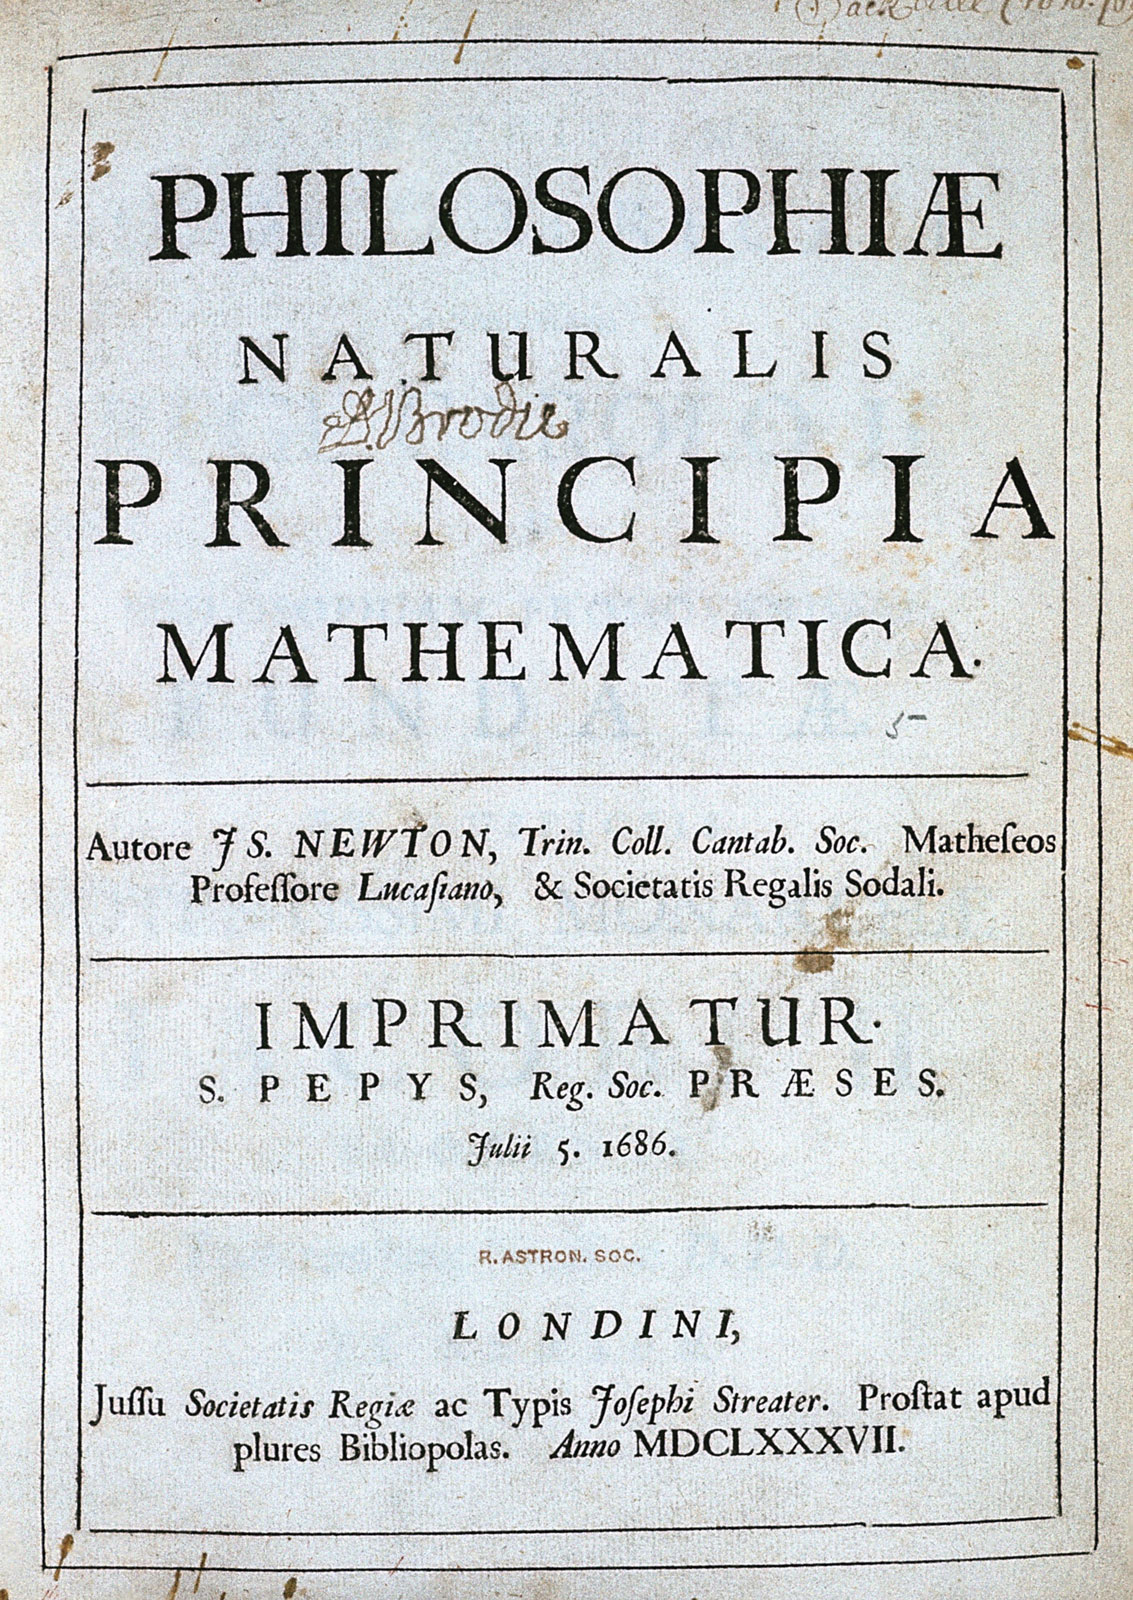
\includegraphics[width=8cm]{nayakn_image1}
    \caption{Sir Isaac Newton's \textit{Principia Mathematica}.}
    \label{fig:1}
\end{figure}

\begin{thebibliography}{2}

\bibitem{} 
Smith, George. “Newton's Philosophiae Naturalis Principia Mathematica.” Stanford Encyclopedia of Philosophy, Stanford University, 20 Dec. 2007, plato.stanford.edu/entries/newton-principia/. 

\bibitem{}
Four Elements: Aristotle, web.lemoyne.edu/~giunta/EA/ARISTOTLEann.html. 

\end{thebibliography}
